\section{Конструкторский раздел}

\subsection{Проектирование базы данных}

В соответствии с диаграммой <<сущность-связь>>, представленной на рисунке \ref{erd}, база данных должна содержать следующие таблицы:

\begin{itemize}[label=---]
	\item таблица текстов text;
	
	\item таблица жанров текстов genre;
	
	\item таблица для связи метаразметки и жанров meta\_genre;
	
	\item таблица метаразметки meta\_annotation;
	
	\item таблица языковых пар language\_pair;
	
	\item таблица предложений sentence;
	
	\item таблица слов word;
	
	\item таблица морфологической аннотации morphological\_annotation;
	
	\item таблица пользователей user;
	
	\item таблица стран country;
	
	\item таблица языков language.
\end{itemize}

Диаграмма проектируемой базы данных представлена на рисунке \ref{er-base}.

\begin{figure}[ht]
	\centering
	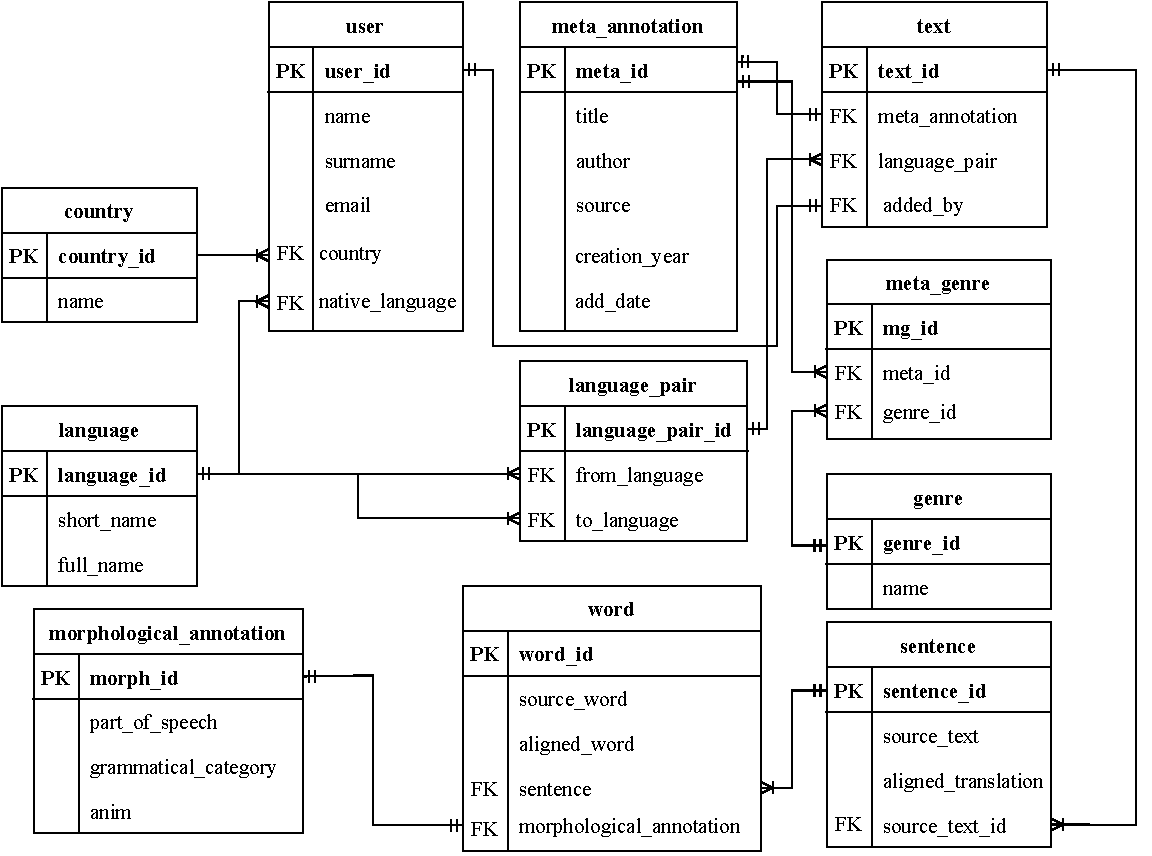
\includegraphics[width=\textwidth]{img/er-base.pdf}
	\caption{Диаграмма БД}
	\label{er-base}
\end{figure}
\pagebreak

Таблица meta\_annotation содержит информацию о метаразметке текста и содержит следующие поля:

\begin{itemize}[label=---]
	\item meta\_id -- уникальный идентификатор записи метаразметки, PK (первичный ключ, англ. primary key), тип данных integer (целое);
	
	\item title -- название текста, string (строка);
	
	\item author -- информация об авторе текста, string (строка); 
	
	\item source -- информация об источнике текста, string (строка);
	
	\item creation\_year -- год создания текста, integer (целое);
	
	\item add\_date -- дата добавления текста в базу данных, date (дата).
\end{itemize}

Информация о жанрах хранится в таблице genre. Она имеет следующие поля: genre\_id -- уникальный идентификатор языка, PK, тип данных integer (целое), name -- имя жанра (например, <<drama>> или <<thriller>>), string (строка).

В таблице language хранится информация о языках, представленных в системе. 
В таблице имеются следующие поля:

\begin{itemize}[label=---]
	\item language\_id -- уникальный идентификатор языка, PK, тип данных integer (целое);
	
	\item short\_name -- сокращенное название языка (например, <<ru>> или <<fr>>), string (строка);
	
	\item full\_name -- полное название языка на английском языке (например, <<Rus-sian>> или <<French>>), string (строка).
\end{itemize}

Информация о языковых парах хранится в таблице language\_pair, которая имеет следующие поля:

\begin{itemize}[label=---]
	\item language\_pair\_id -- уникальный идентификатор языка, PK, тип данных\\ integer (целое);
	
	\item from\_language -- исходный язык (с которого производится перевод), FK (внешний ключ, англ. foreign key) на поле language\_id таблицы language, integer (целое);
	
	\item to\_language -- целевой язык (на который производится перевод), FK на поле language\_id таблицы language, integer (целое).
\end{itemize}

Хранящиеся в базе тексты представлены в таблице text со следующими полями:

\begin{itemize}[label=---]
	\item text\_id -- уникальный идентификатор текста, PK, тип данных integer (целое);
	
	\item meta\_annotation -- информация о метаразметке, FK на поле meta\_id таблицы meta\_annotation, integer (целое);
	
	\item language\_pair -- информация о направлении перевода (исходном и целевом языках текстов), FK на поле language\_pair\_id таблицы language\_pair, integer (целое).
	
	\item added\_by -- указание на пользователя, который добавил текст, FK на поле user\_id таблицы user, uuid.
\end{itemize}

Поскольку метаразметка и жанры связаны связью <<многие-ко-многим>>, необходимо формализовать её с помощью дополнительной таблицы meta\_genre, которая имеет следующие поля:

\begin{itemize}[label=---]
	\item mg\_id -- уникальный идентификатор отношения текста и жанра, PK, тип данных integer (целое);
	
	\item meta\_id -- идентификатор метаразметки, FK на поле meta\_id таблицы \\meta\_annotation, тип данных integer (целое);
	
	\item genre\_id -- идентификатор жанра, FK на поле genre\_id таблицы genre, тип данных integer (целое);
\end{itemize}

Информация о выровненных предложениях хранится в таблице sentence, имеющей следующие поля:

\begin{itemize}[label=---]
	\item sentence\_id -- уникальный идентификатор предложения, PK, тип данных integer (целое);
	
	\item source\_text -- предложение на исходном языке, string (строка);
	
	\item aligned\_translation -- перевод предложения, string (строка);
	
	\item source\_text\_id -- идентификатор текста, из которого взято предложение, FK на поле text\_id таблицы text, integer (целое).
\end{itemize}

Вся морфологическая разметка слов содержится в таблице morphologi-cal\_annotation, которая имеет следующие поля:

\begin{itemize}[label=---]
	\item morph\_id -- уникальный идентификатор морфологической аннотации, PK, тип данных integer (целое);
	
	\item part\_of\_speech - часть речи, string (строка);
	
	\item grammatical\_category -- грамматическая категория, string (строка);
	
	\item anim -- одушевленность слова, string (строка).
\end{itemize}

В таблице word хранится информация о выровненных парах слов: слову на изначальном языке приписывается его перевод и морфологические признаки слова (в исходном языке). 
Таблица word содержит следующие поля:

\begin{itemize}[label=---]
	\item word\_id -- уникальный идентификатор слова, PK, тип данных integer (целое);
	
	\item source\_word -- слово на исходном языке, string (строка);
	
	\item aligned\_word -- выровненный перевод слова, string (строка);
	
	\item sentence -- идентификатор предложения, из которого взято слова (его контекст), FK на поле sentence\_id таблицы sentence, integer (целое);
	
	\item morphological\_annotation -- идентификатор морфологической разметки\\ слова, FK на поле morpho\_id таблицы morphological\_annotation, integer (целое).
\end{itemize}

Что касается пользователей, необходимо сначала рассмотреть способ хранения стран в базе данных. 
Для этого используется таблица country с полями country\_id -- уникальный идентификатор страны, PK, тип данных integer (целое) и name -- название страны, string (строка).

Наконец, информация о пользователях базы хранится в таблице user со следующими полями:

\begin{itemize}[label=---]
	\item user\_id -- уникальный идентификатор пользователя, PK, тип данных uuid;
	
	\item name -- имя пользователя, строка (string);
	
	\item surname -- фамилия пользователя, строка (string);
	
	\item email -- электронный адрес пользователя, строка (string);
	
	\item country -- страна пользователя, FK на поле country\_id таблицы country, integer (целое);
	
	\item native\_language -- родной язык пользователя, FK на поле language\_id таблицы language, integer (целое).
\end{itemize}

\subsection{Ограничения целостности базы данных}

Для поддержания целостности базы данных введены ограничения на некоторые атрибуты. Разработанные ограничения представлены в таблице~\ref{integrity}. Первичный ключ обозначен как PK (данные в столбце уникальны и не null), внешний ключ как FK (должна существовать запись в другой таблице с внешним ключом в качестве значения указанного атрибута).

\begin{table}[H]
	\caption{Ограничения целостности базы данных}\label{integrity}
	\begin{tabular}{|c|c|c|}
		\hline
		Таблица                           & Атрибут                                                               & Ограничение                \\ \hline
		\multirow{4}{*}{text}             & text\_id                                                              & PK                         \\ \cline{2-3} 
		& meta\_annotation                                                      & FK                         \\ \cline{2-3} 
		& language\_pair                                                       & FK                         \\ \cline{2-3} 
		& added\_by                                                             & FK                         \\ \hline
		\multirow{3}{*}{meta\_genre}      & mg\_id                                                                & PK                         \\ \cline{2-3} 
		& meta\_id                                                              & FK                         \\ \cline{2-3} 
		& genre\_id                                                             & FK                         \\ \hline
		genre                             & genre\_id                                                             & PK                         \\ \hline
		\multirow{2}{*}{sentence}         & sentence\_id                                                          & PK                         \\ \cline{2-3} 
		& text\_id                                                              & FK                         \\ \hline
		\multirow{3}{*}{word}             & word\_id                                                              & PK                         \\ \cline{2-3} 
		& sentence\_id                                                          & FK                         \\ \cline{2-3} 
		& \begin{tabular}[c]{@{}c@{}}morpholo-\\ gical\_annotation\end{tabular} & FK                         \\ \hline
		morphological\_annotation         & morph\_id                                                             & PK                         \\ \hline
		language                          & language\_id                                                          & PK                         \\ \hline
		\multirow{3}{*}{language\_pair}   & language\_pair\_id                                                    & PK                         \\ \cline{2-3} 
		& from\_language                                                        & FK                         \\ \cline{2-3} 
		& to\_language                                                          & FK                         \\ \hline
		country                           & country\_id                                                           & PK                         \\ \hline
		\multirow{3}{*}{user}             & user\_id                                                              & PK                         \\ \cline{2-3} 
		& country                                                               & FK                         \\ \cline{2-3} 
		& native\_language                                                      & FK                         \\ \hline
		\multirow{3}{*}{meta\_annotation} & meta\_id                                                              & PK                         \\ \cline{2-3} 
		& creation\_year                                                        & От 1700 до текущ. года     \\ \cline{2-3} 
		& add\_date                                                             & От мая 2023 до текущ. даты \\ \hline
	\end{tabular}
\end{table}\pagebreak

\subsection{Разработка алгоритмов}

Основная цель базы данных -- поиск слов с их переводом и примерами употребления. 
Схема базового алгоритма поиска слова в корпусе (без фильтров) представлена на рисунке~\ref{basic-search}.

\begin{figure}[ht]
	\centering
	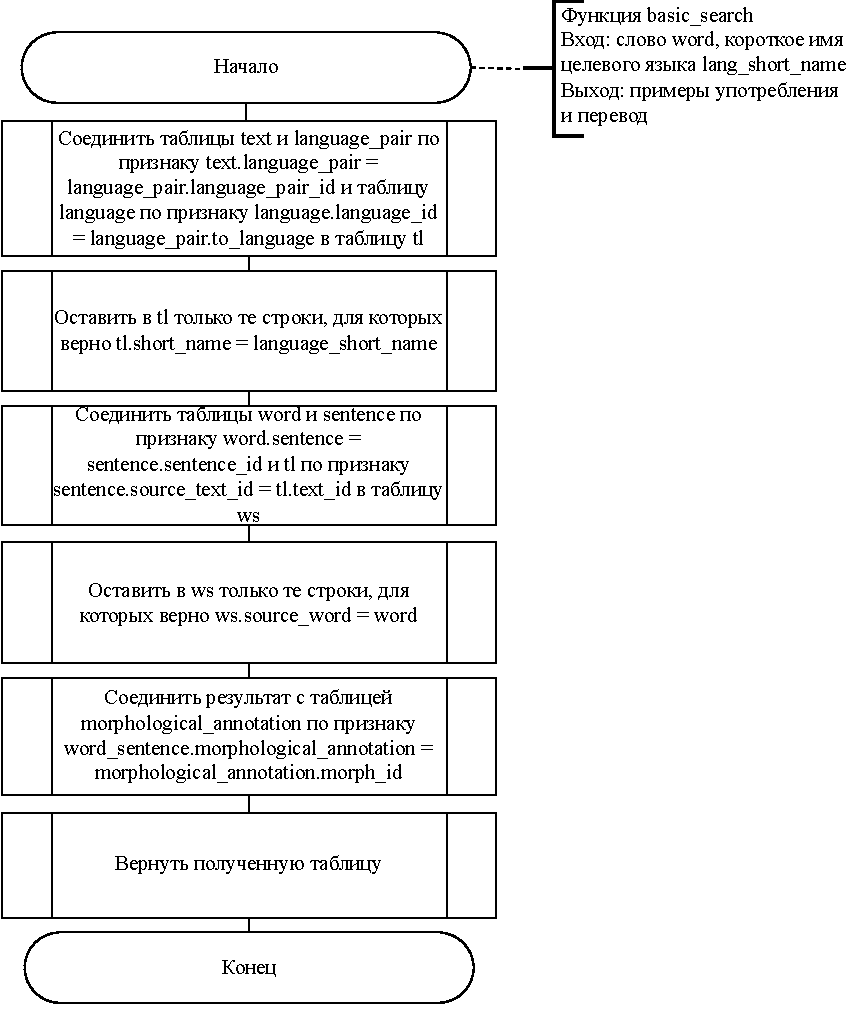
\includegraphics[scale=1]{img/search-algo-basic.pdf}
	\caption{Схема базового алгоритма поиска}
	\label{basic-search}
\end{figure}\clearpage

Схема алгоритма поиска слова в корпусе среди текстов указанного автора, представлена на рисунке~\ref{author-search}.

\begin{figure}[ht]
	\centering
	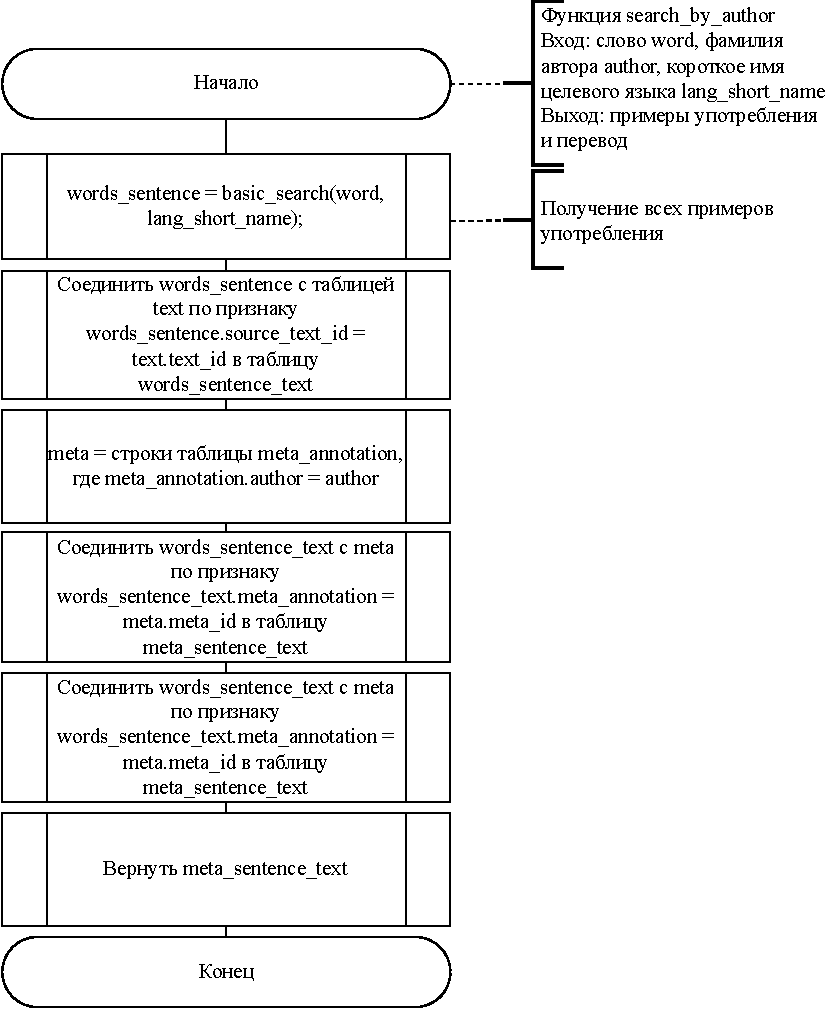
\includegraphics[scale=1]{img/search-algo-author.pdf}
	\caption{Схема алгоритма поиска слова в текстах автора}
	\label{author-search}
\end{figure}\clearpage

Схема алгоритма поиска примеров употребления слова в корпусе по дате добавления текста представлена на рисунке~\ref{date-search}.

\begin{figure}[ht]
	\centering
	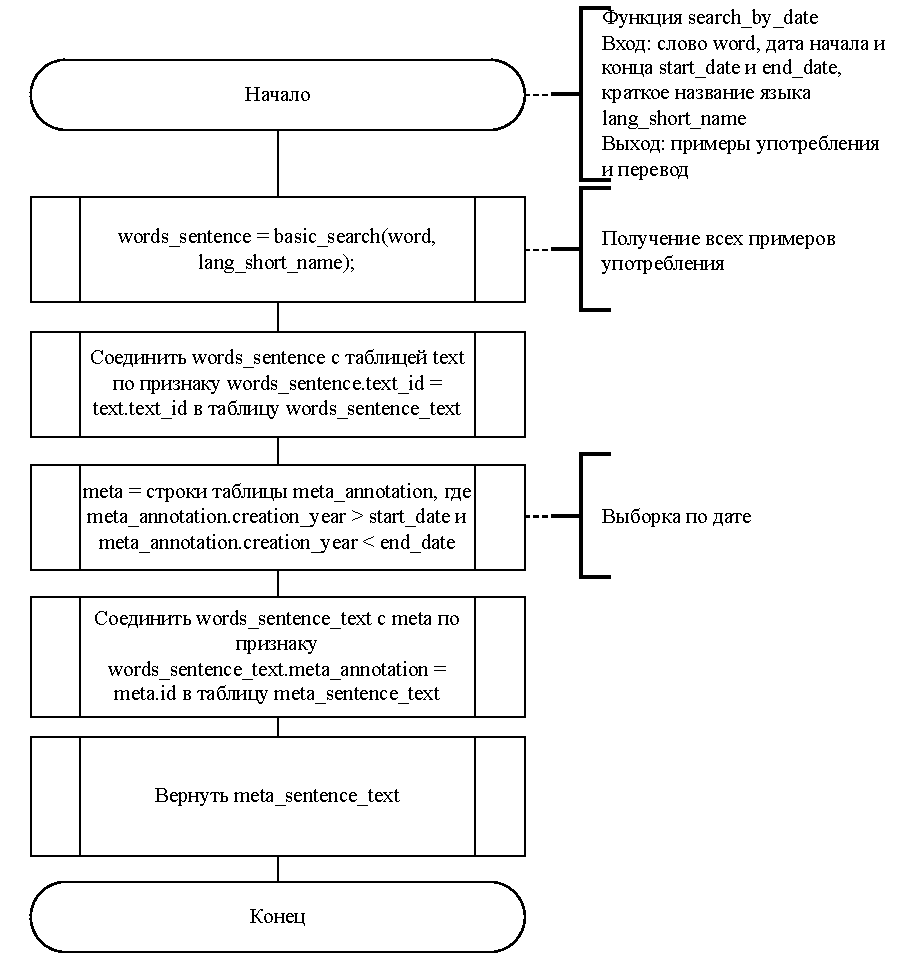
\includegraphics[width=\textwidth]{img/search-algo-date.pdf}
	\caption{Схема алгоритма поиска слова в текстах по дате}
	\label{date-search}
\end{figure}
\clearpage
Схема алгоритма поиска с учетом заданной части речи представлена на рисунке~\ref{pos-search}.

\begin{figure}[ht]
	\centering
	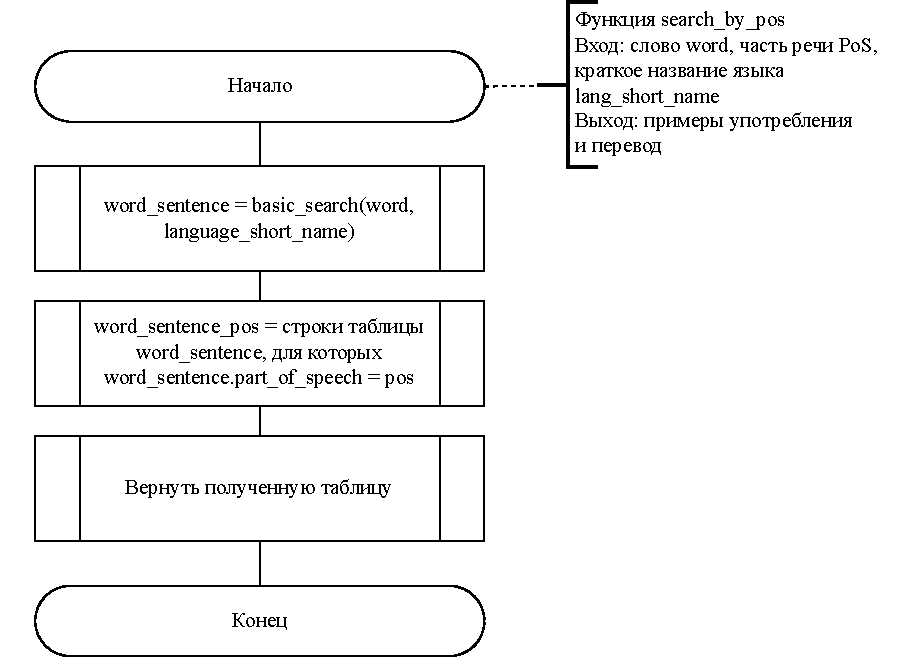
\includegraphics[width=\textwidth]{img/search-algo-pos.pdf}
	\caption{Схема алгоритма поиска слова с учетом заданной части речи}
	\label{pos-search}
\end{figure}

Алгоритмы поиска по другим морфологическим признакам строятся аналогично (функции search\_by\_anim, search\_by\_gram).
\clearpage

Схема алгоритма поиска слова в корпусе среди текстов заданного жанра представлена на рисунке~\ref{genre-search}.

\begin{figure}[ht]
	\centering
	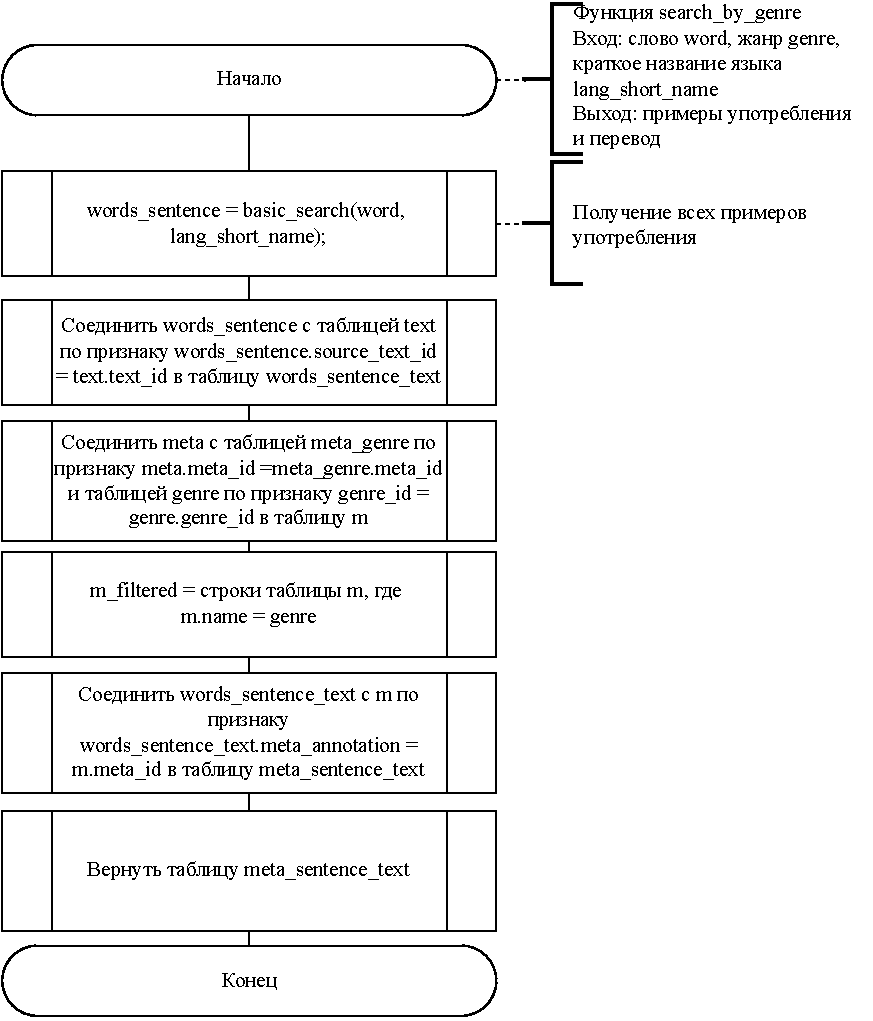
\includegraphics[scale=1]{img/search-algo-genre.pdf}
	\caption{Схема алгоритма поиска слова с учетом заданного жанра текстов}
	\label{genre-search}
\end{figure}
\clearpage

%Схема обобщенного алгоритма поиска по заданным фильтрам представлен на рисунках %\ref{common-search-1} -- \ref{common-search-3}.

%\begin{figure}[ht]
%	\centering
%	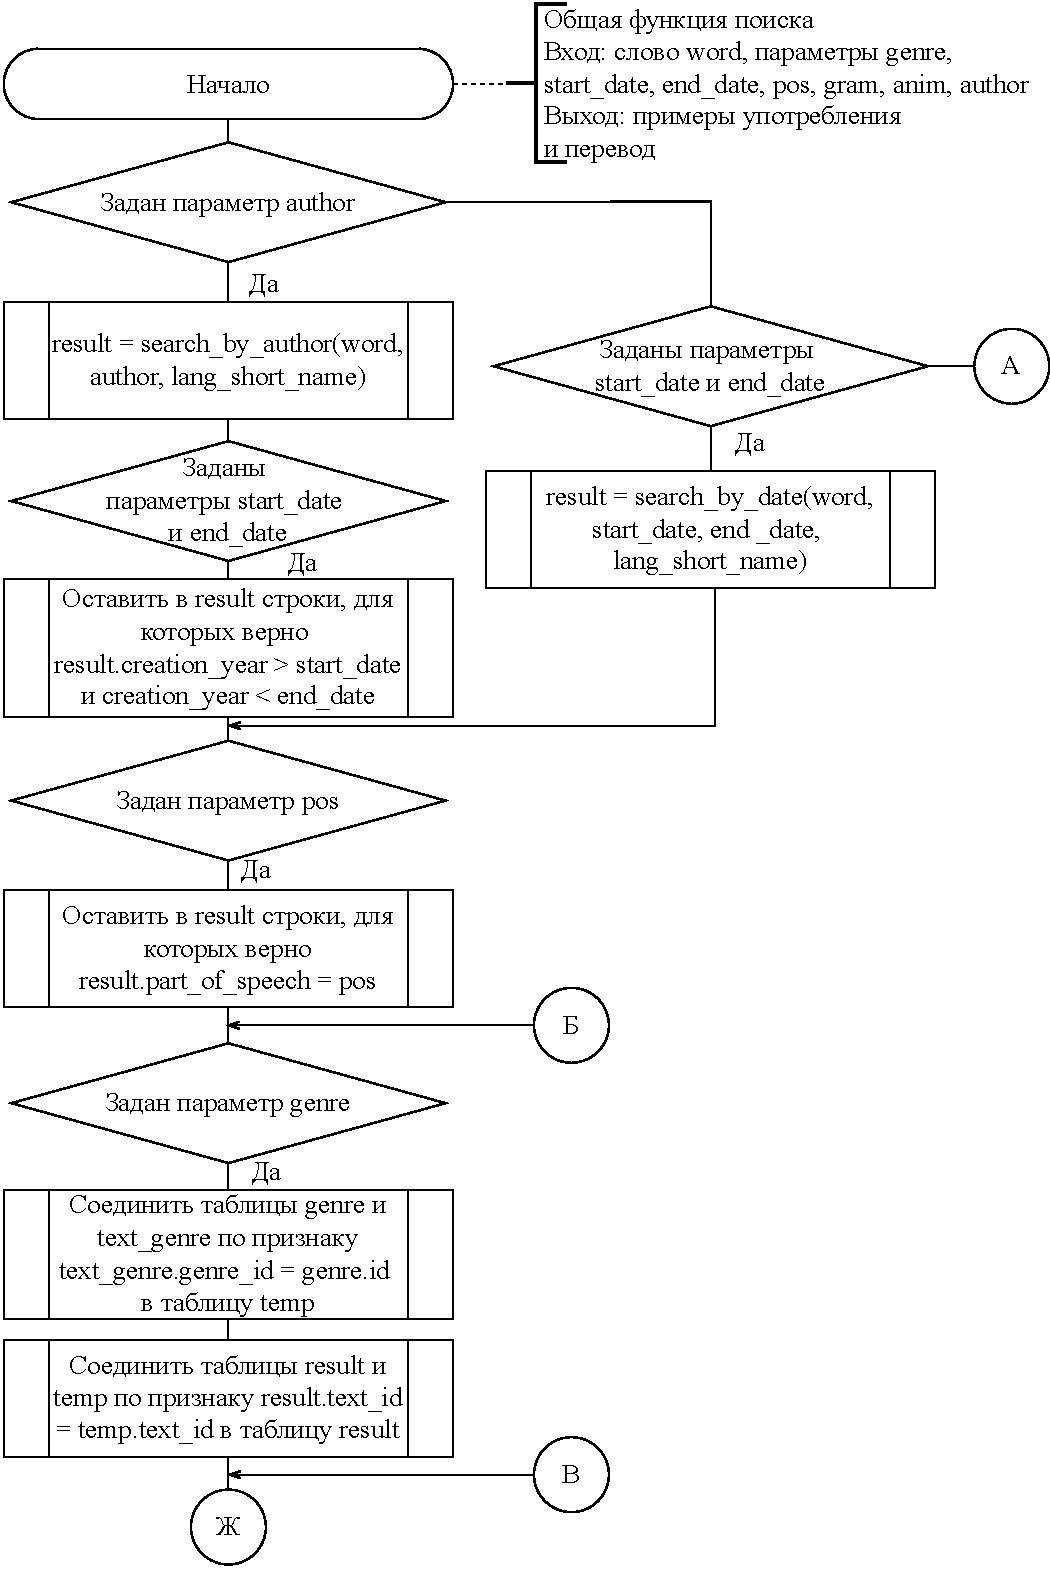
\includegraphics[scale=0.7]{img/search-algo-common-1.pdf}
%	\caption{Схема обобщенного алгоритма поиска по заданным фильтрам, ч.1}
%	\label{common-search-1}
%\end{figure}

%\begin{figure}[ht]
%	\centering
%	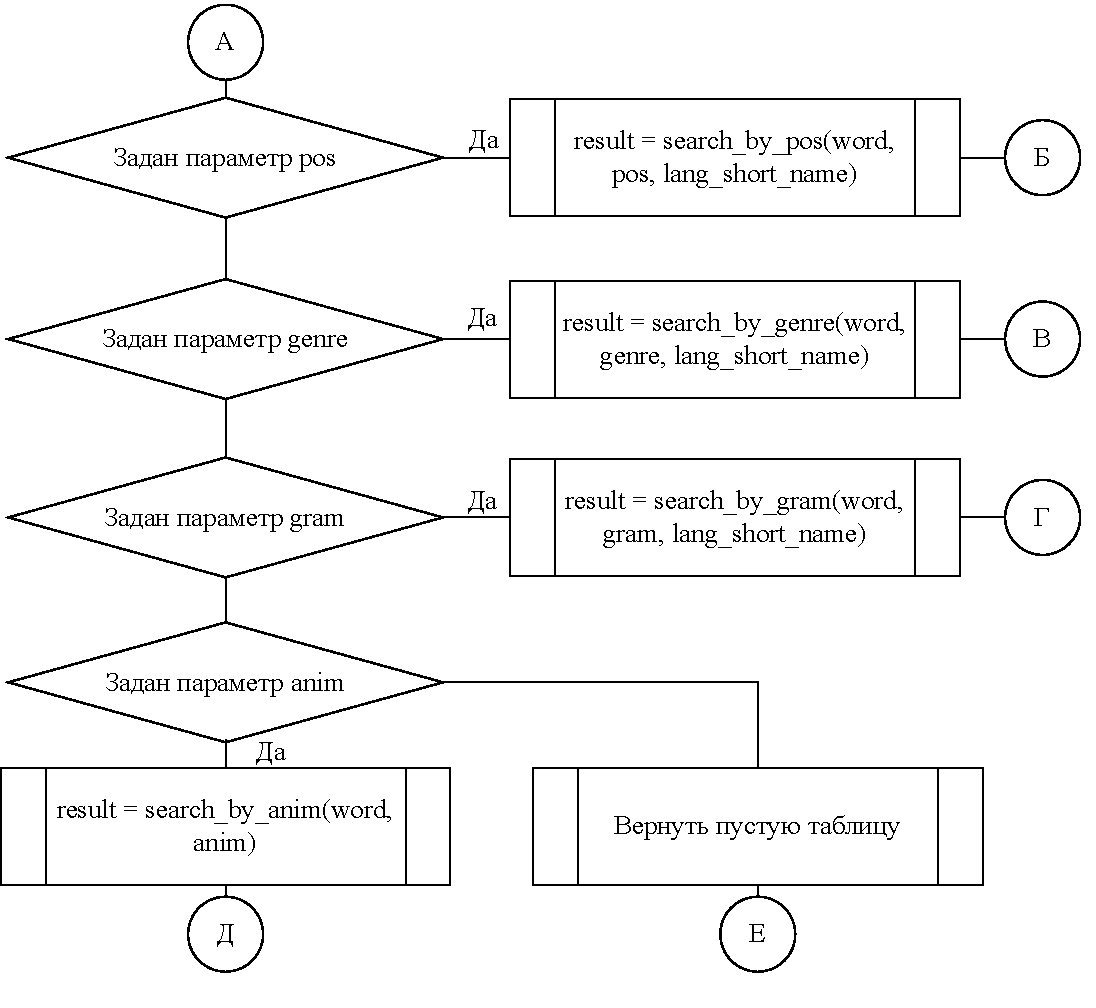
\includegraphics[scale=0.6]{img/search-algo-common-2.pdf}
%	\caption{Схема обобщенного алгоритма поиска по заданным фильтрам, ч.2}
%	\label{common-search-2}
%\end{figure}

%\begin{figure}[ht]
%	\centering
%	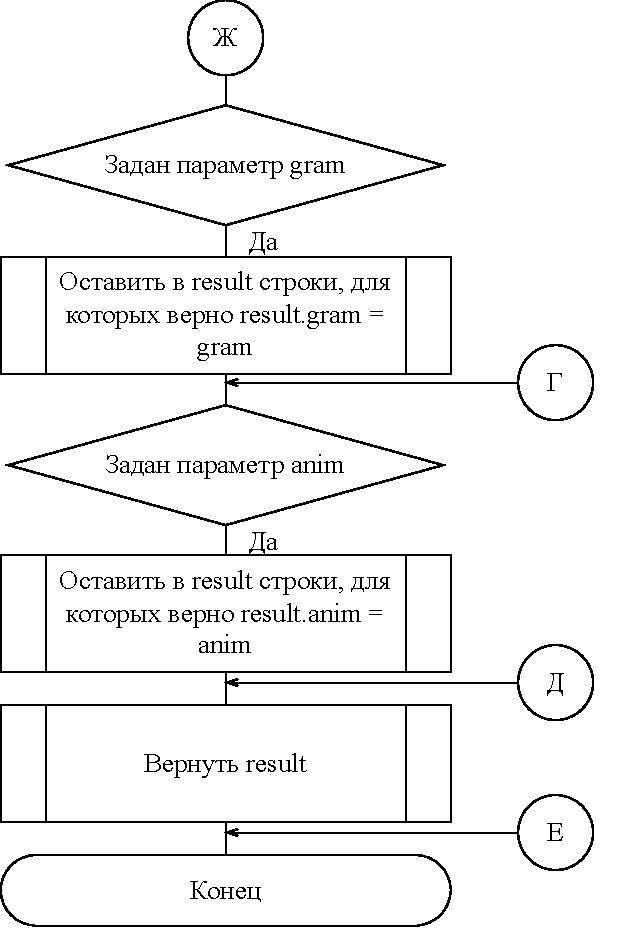
\includegraphics[scale=0.6]{img/search-algo-common-3.pdf}
%	\caption{Схема обобщенного алгоритма поиска по заданным фильтрам, ч.3}
%	\label{common-search-3}
% \end{figure}
% \clearpage

\subsection{Проектирование кеширования запросов}

Как видно из схем спроектированных алгоритмов, для каждого запроса необходимо выполнять определенное количество соединений таблиц, что является трудоемкой задачей. 
Поэтому, для исключения повторных вычислений и, соответственно, ускорения поиска, рационально использовать дополнительную кеширующую базу данных.
В этом хранилище необходимо сохранять результаты запросов и собственно сами запросы, чтобы можно было потом найти ранее вычисленный результат.
Запрос можно сохранять в виде структуры: слово и фильтры. 
Слово -- строка.
Фильтры задаются набором полей, которые могут быть null (поскольку не в каждом запросе заданы все параметры).
Результат также задается в формате структуры (словарь или таблица -- в зависимости от формата хранения данных).
Кеш будет становиться недействительным по истечении 24 часов.
Таким образом, ключи будут иметь следующий формат: \{слово\}-\{язык\}-\{жанр\}-\{время начала\}-\{время конца\}-\{часть речи\}-\{грамм. категория\}-\{одушевлен-ность\}-\{автор\}.

\subsection{Проектирование компонентов системы}

Диаграмма компонентов проектируемой системы в нотации UML представлена на рисунке~\ref{components}.

\begin{figure}[ht]
	\centering
	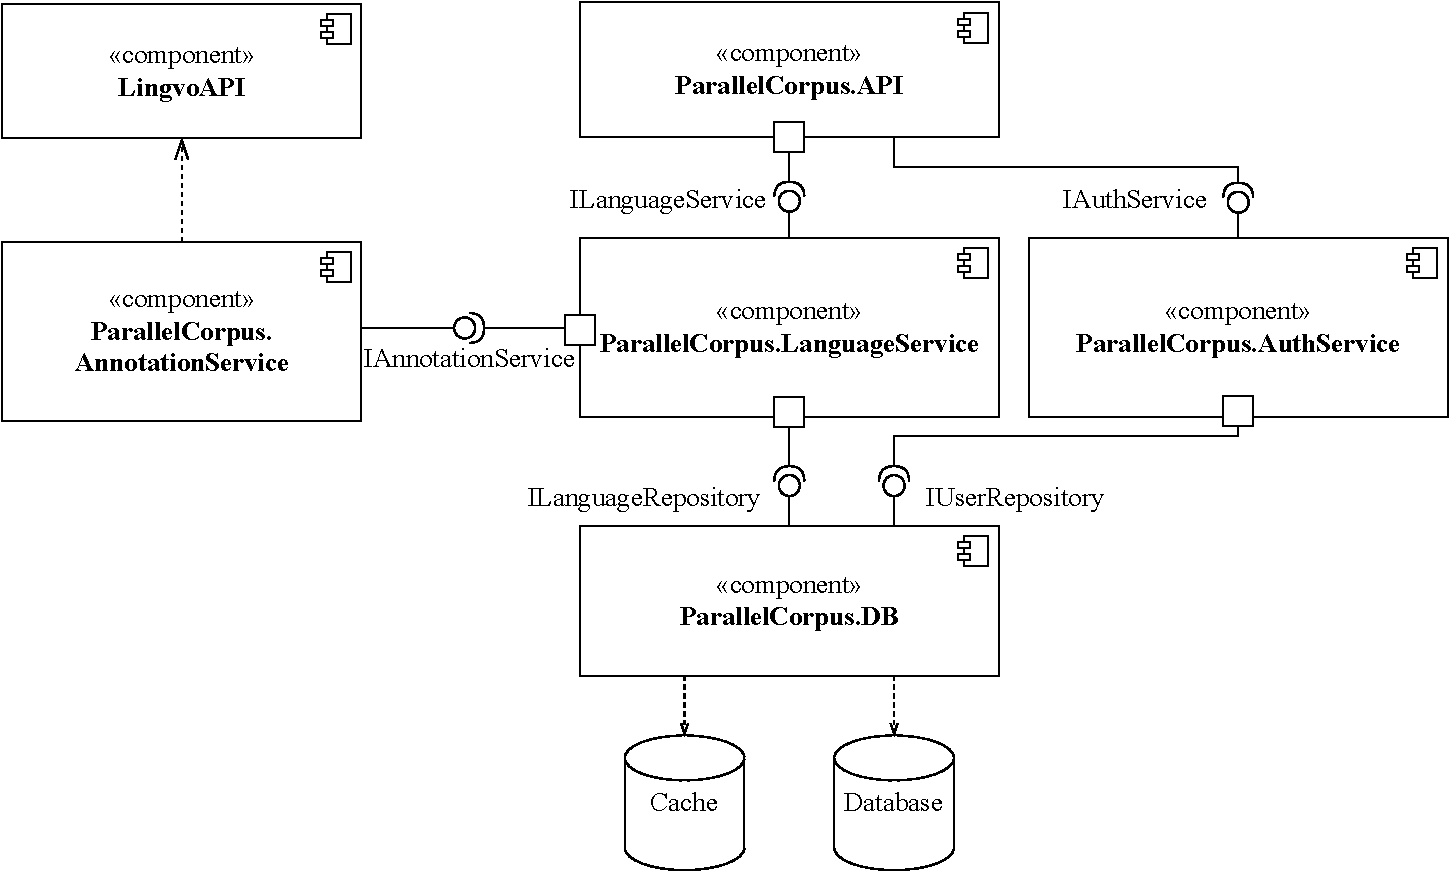
\includegraphics[scale=0.7]{img/components.pdf}
	\caption{Диаграмма компонентов системы}
	\label{components}
\end{figure}\pagebreak

Система разрабатывается для хранения и пополнения параллельного корпуса текстов на естественных языках. Таким образом, выделяются следующие компоненты: 
ParallelCorpus.LanguageService, реализующий все возможные действия с корпусом через интерфейс ILanguageService,
ParallelCorpus.Annotati-onService, отвечающий за разметку текстов. Взаимодействие других компонентов с ParallelCorpus.AnnotationService осуществляется через интерфейс IAnnota-tionService. При этом, этот компонент является оберткой для функций компонента LingvoAPI обработки лингвистических данных.

Поскольку в системе также разграничиваются типы пользователей и присутствует функционал регистрации, выделяется сервис авторизации ParallelCor-pus.AuthService, взаимодействие с которым осуществляется с помощью интерфейса IAuthService.

Все действия приложения с данными реализованы в компоненте Paral-lelCorpus.DB. Он предоставляет интерфейс для взаимодействия с помощью интерфейсов ILanguageRepository и IUserRepository, отвечающих за данные корпуса и пользователей соответственно.

За взаимодействие пользователей (клиентов) с системой отвечает компонент ParallelCorpus.API.

\subsection{Протоколирование}

Протоколирование (логирование) событий, происходящих в системе, позволяет разработчикам, в случае возникновения ошибок, воспроизводить и оперативно их устранять. 
Для того, чтобы это было возможным, необходимо обеспечить достаточную детализацию происходящих действий. 
Это достигается протоколированием всех действий пользователя, в том числе запросов к базе данных с указанием используемых данных. 
Однако необходимо принять во внимание, что такое подробное логирование может привести, во-первых, к увеличению потребляемой памяти, и, во-вторых, к протоколированию чувствительных данных \cite{wilkins-logging-2022}. 
Первая проблема решается конфигурированием уровня логирования, вторая -- внимательным отслеживанием данных, передающихся в логи. 

Для данной системы выбраны следующие события, которые необходимо логировать:

\begin{itemize}[label=---]
	\item все внешние запросы к системе с указанием id пользователя, запрашиваемого сервиса и передаваемых данных;
	\item добавление, удаление, извлечение и изменение данных в базе данных;
	\item все вызовы сторонних сервисов (например, сервиса обработки лингвистических данных) с указанием вызываемого функционала и передаваемых данных;
	\item ответы на запросы к базе данных и компонентам системы;
	\item все ошибки, исключения и коды возврата.
\end{itemize}

\subsection{Проектирование ролевой модели}

Ранее введены следующие роли: неавторизованный пользователь, преподаватель, переводчик и администратор.

Неавторизованный пользователь не имеет доступа ни к каким таблицам, кроме таблицы user, в которую он может добавлять данные для обеспечения возможности регистрации и авторизации.

Администратор, напротив, имеет доступ ко всем таблицам на их чтение, а также на изменение, удаление и добавление в них данных.

Переводчик имеет права на чтение, добавление, изменение и удаление данных из таблиц text, genre, text\_genre, sentence, word, morphological\_annotation, meta\_annotation. 
Причем изменение и удаление возможно только для тех данных, которые ранее были добавлены данным пользователем. Доступ переводчика к таблицам language, country и language\_pair возможен только для чтения.

Роль преподавателя отличается от переводчика отсутствием прав на добавление, изменение и удаление информации в таблицах text, genre, text\_genre, sentence, word, morphological\_annotation, meta\_annotation -- однако возможность чтения информации сохраняется.

Никто, кроме администратора, не имеет права изменять структуру таблиц, удалять их или добавлять новые таблицы.

\subsection*{Вывод}

В данном разделе представлена диаграмма проектируемой базы данных. 
Для формализации отношения <<многие-ко-многим>> выделена дополнительная сущность. Для всех таблиц описаны их атрибуты. 
Кроме того, описаны ограничения целостности базы данных: в каждой таблице выделен первичный ключ, описаны внешние ключи, а также описана необходимая валидация для некоторых полей.

Разработан алгоритм функции поиска как без фильтров, так и по каждому фильтру. Также в виде схемы представлен обобщенный алгоритм поиска, объединяющий все функции.

Описан требуемый формат кеширования данных: необходимо сохранение как запроса, так и результата. Кеширование позволит избежать повторных соединений таблиц для одного и того же запроса. Также описаны события в системе, которые необходимо записывать в журнал: это все запросы пользователя, ответы на них, запросы к базе данных и все ошибки в системе.

Представлена диаграмма компонентов приложения к базе данных, в которую включены компоненты обработки запросов, выравнивания текстов и морфологической разметки слов.

Наконец, спроектирована ролевая модель на уровне базы данных. 
Для каждой из выделенных ролей: неавторизованный пользователь, переводчик, преподаватель и администратор, описаны права доступа к таблицам базы данных.



\pagebreak